\documentclass[report.tex]{subfiles} 
\begin{document}
\section{Key Schedule Expansion} \label{key schedule}

The AES standard uses a cipher key which is determined by the implementers or users of the standard and a key schedule to compute the rest of the keys used in the encryption process. %\cite[Sec.~5]{AES Standard}
The predetermined cipher key is used in the first iteration and the round keys are used from the second iteration to the final iteration.

The round keys have the same length as the original cipher and are all generated by information on the former round key. The key expansion process is divided into four different parts: word rotation, word substitution, round constant addition and the procedure of generation.

\subsection{Word Rotation}
The Word Rotation function is a cyclic single right byte shift where the least significant byte is shifted to the place of the most significant byte. Figure \ref{fig:word shift} shows this function graphically.

\begin{figure}[ht]
\setlength{\unitlength}{1.0cm}
	\begin{center}
		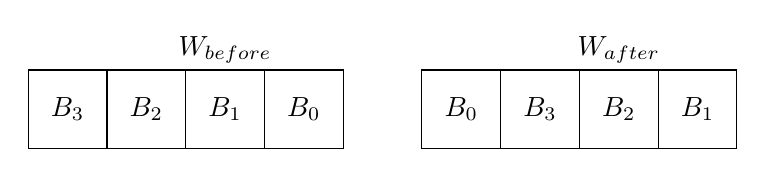
\begin{tikzpicture}
			\foreach \x/\B in {0/3,1/2,2/1,3/0}
				{
					\node[draw, shape=rectangle, minimum height=1cm, minimum width=1cm, inner sep=0] () at (\x,0){$B_{\B}$};	
				}
				\node () at (2, 0.75){$W_{before}$};
			\foreach \x/\B in {5/0,6/3,7/2,8/1}
				{
					\node[draw, shape=rectangle, minimum height=1cm, minimum width=1cm, inner sep=0] () at (\x,0){$B_{\B}$};	
				}
				\node () at (7, 0.75){$W_{after}$};
				

		\end{tikzpicture}
	\end{center}
	\caption{Graphical interpretation of the word rotation function.}
	\label{fig:word shift}
\end{figure}

\subsection{Round Constant Array}
The round constant array is defined as a word array where the least significant byte is defined as
\begin{equation}
	\textrm{rcon}\left(i\right) = x^{i - 1}
\end{equation}
and the other bytes is filled with zeros and where $x^{i - 1}$ is calculated using the multiplication defined in  \ref{sec:multiplication} and i denotes the round. A figure showing the interesting bytes of this array is given in Figure \ref{fig:round constant array}.

\begin{figure}[ht]
\setlength{\unitlength}{1.0cm}
	\begin{center}
		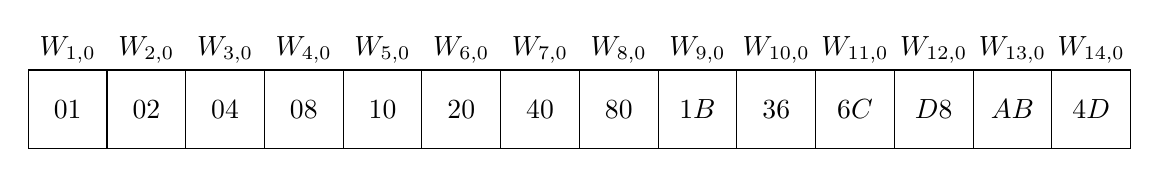
\begin{tikzpicture}
			\foreach \x/\B in {1/01,2/02,3/04,4/08,5/10,6/20,7/40,8/80, 9/1B, 10/36, 11/6C, 12/D8, 13/AB, 14/4D}
				{
					\node[draw, shape=rectangle, minimum height=1cm, minimum width=1cm, inner sep=0] () at (\x,0){$\B$};
					\node () at (\x, 0.75){$W_{\x,0}$};
				}
		\end{tikzpicture}
	\end{center}
	\caption{Least significant byte row of the round constant array.}
	\label{fig:round constant array}
\end{figure}
Note that the length of the array is determined of the length of the encryption.

\subsection{Word Substitution}
	The word substitution process follows the same pattern as in\ref{sec:substitution} and every byte in the word is substituted according to the look up table given in \ref{fig:s-box}.
	
\subsection{Round Key Generation}
	With all the components of the round key generation process described can the algorithm be described.
\end{document}
